\documentclass[pldi]{sigplanconf-pldi15}
% Requires temporary version of sigplanconf style file provided on
% PLDI'15 web site.

%\def\inlinecode{\code}
%\def\code{\lstinline[basicstyle=\ttfamily]}
\newcommand{\code}[1]{\mintinline{c}{#1}}

\usepackage{supertech}
\usepackage[binary]{SIunits}            % typset units correctly
\usepackage{courier}            % standard fixed width font
\usepackage[scaled]{helvet} % see www.ctan.org/get/macros/latex/required/psnfss/psnfss2e.pdf
\usepackage[hyphens]{url}                  % format URLs

\ifnotes
\newcommand{\bcknote}[1]{\cnote{red}{#1}{bck}}
\else
\fi

% Try \usepackage[hyphens]{url}
% or try this
%% \makeatletter
%% \g@addto@macro{\UrlBreaks}{\UrlOrds}
%% \makeatother

%\usepackage{listings}          % format code
\usepackage{enumitem}      % adjust spacing in enums
\usepackage[colorlinks=true,allcolors=blue,breaklinks,draft=false]{hyperref}   % hyperlinks, including DOIs and URLs in bibliography
\newcommand{\doi}[1]{doi:~\href{http://dx.doi.org/#1}{\Hurl{#1}}}   % print a hyperlinked DOI

\usepackage{minted}
%\usepackage{pslatex}
\usepackage{graphicx}
%\usepackage{wrapfig}
%\usepackage{dblfloatfix}

%\newcommand{\figref}[1]{Figure~\ref{fig:#1}}
%\newcommand{\punt}[1]{}

%\usepackage{titling}             % Uncomment both to   
%\setlength{\droptitle}{-2em}     % change title position 

\newcommand{\ns}[1]{\unit{#1}\nano\second{}}

\begin{document}
\special{papersize=8.5in,11in}% Still need this even with letterpaper
\title{SuperMalloc: A Super Fast Multithreaded \texttt{malloc()} for 64-bit Machines}
%\author{Bradley C. Kuszmaul \hspace{0.2in} \texttt{bradley@mit.edu}}
\date{}
\maketitle
\begin{abstract}
SuperMalloc is an implementation of \texttt{malloc(3)} originally
designed for X86 Hardware Transactional Memory (HTM)\@.  It turns out
that the same design decisions also make it fast even without HTM\@.
We compared SuperMalloc to DLmalloc, JEmalloc, Hoard, and TBBmalloc,
For the malloc-test benchmark, with one thread SuperMalloc is about
2.1 times faster than the best alternatives, with 8 threads and HTM
SuperMalloc is 2.75 times faster, and on 32 threads without HTM
SuperMalloc is 3.4 times faster.  SuperMalloc generally compares
favorably with the other allocators on speed, scalability, speed
variance, memory footprint, and code size.

SuperMalloc achieves these performance advantages using less than half
as much code as the alternatives.  We exploit the fact that although
physical memory is always precious, virtual address space on a 64-bit
machine is relatively cheap.  We allocate \unit{2}\mebi\byte{} chunks
which contain objects all the same size.  To translate chunk numbers
to chunk metadata, we use a simple array (most of which is uncommitted
to physical memory).  We take care to avoid associativity conflicts in
the cache: most of the size classes are a prime number of cache lines,
and nonaligned huge accesses are randomly aligned within a page.
Objects are allocated from the fullest non-full page in the
appropriate size class.  For each size class, we employ a 10-object
per-thread cache, a per-CPU cache that holds up a few megabytes per
size class, and a global cache that is organized so we can move about
a megabyte between a per-CPU cache and the global cache using $O(1)$
instructions.  We prefetch everything we can before starting a
critical section, which makes the critical sections run fast, and for
HTM improves the odds that the transaction will commit.

\end{abstract}

\secput{intro}{Introduction}

C/C++ dynamic memory allocation functions (\code{malloc(3)} and
\code{free(3)}) can impact the cost of running applications.  The cost
can show up in several ways: allocation operations can be slow for
serial programs, they can fail to scale with the number of cores in a
multithreaded multicore environment, they can occasionally be slow,
and they can induce a large memory footprint.  Furthermore, if the
allocator itself is too complex, it can inhibit improvements.  We can
divide these problems roughly into three categories: speed, footprint,
and complexity. 

The rest of this section explores this space in the context of several
allocators.  The allocators include DLmalloc~\cite{Lea96},
Hoard~\cite{BergerMcBl00}, JEmalloc~\cite{Evans06},
TBBmalloc~\cite{KukanovVo07}, and our allocator, SuperMalloc.
\figref{codesize} shows the code size for the allocators, including
our allocator, SuperMalloc.

Many modern allocators take advantage of the fact that the operating
system allocates memory in two steps corresponding to virtual
allocation and physical allocation: First a system call such as
\code{mmap()} allocates a contiguous range of virtual addresses.  At
this point, no physical memory has been allocated.  Later, when the
application actually touches the virtual addresses, a page fault
occurs, and the operating system allocates physical memory.  A page of
virtual memory that has physical memory associated with it is called a
\defn{committed} page, whereas if no physical memory is allocated, the
page is \defn{uncommitted}.  An application or library can use
\code{madvise()} to uncommit a committed page, returning the
underlying physical memory back to the operating system.

{\paragraph{DLmalloc}} \cite{Lea96} is the default single-threaded
allocator in Linux.  DLmalloc is relatively simple and has been stable
for decades.  DLmalloc employs per-object boundary tags (which are due
to~\cite{Knuth73}).  On a 64-bit machine, each allocated object is
immediately preceded by 8 bytes which indicate the size of the object
(and hence the address of the next object, as well as whether the
object is allocated or free, and whether the previous object is
allocated or free.  When the previous object is free, the last 8 bytes
of that object also indicate the size.  When DLmalloc frees an object,
it can immediately coalesce the object with the next object (if it is
free) since it knows the size of the newly freed object.  If the
previous object is freed, it can also coalesce the newly freed object
with the previous one.  The boundary tags can contribute up to a 50\%
space overhead when allocating small (8-byte) objects.  DLmalloc
employs a first-fit heuristic, and has no provision for multithreading
performance beyond using a single lock to protect the entire
allocation data structure.  For example, DLmalloc has no per-thread
caching.

DLmalloc has been placed in the public domain.

{\paragraph{Hoard}} \cite{BergerMcBl00} was introduced during the era
of the first multithreaded allocators.  The original Cilk
allocator~\cite{BlumofeLe94} and the STL allocator of the
time~\cite{SGI97} provided per-thread allocation, which was very fast
(no locking was required), but also produced unbounded memory blowups.
Some allocators, such as PTmalloc~\cite{Gloger06} and
LKmalloc~\cite{LarsonKr98} exhibit memory blowup bounded by $P$, the
number of processors.  Hoard provides a provable bound on its space
blowup.  Hoard organizes small objects into \defn{chunks}, which
contain objects all the same size.\footnote{Chunks are called
  ``superblocks'' in \cite{BergerMcBl00}.  They are called ``chunks''
  in \cite{Evans06} and \cite{KukanovVo07}.}  (Large objects are dealt
with using heavier-weight mechanisms).  Hoard puts metadata at the
beginning of each superblock indicating the size of the objects in the
superblock.  Since the objects within a superblock are all the same,
Hoard does not need boundary tags.

Hoard uses an \defn{allocate-fullest} heuristic.  Hoard sometimes
finds itself in a situation where an object could be allocated out of
any one of several superblocks.  Hoard allocates the object out of the
fullest such superblock. By allocating into the fullest superblock,
Hoard improves the chances that a superblock will completely empty and
can be uncommitted or reused for other purposes.

Hoard is licensed under GPLv2.

\begin{figure}
\begin{center}
\begin{tabular}{lrr}
Allocator & Bytes        & LoC \\ \hline
 DLmalloc    \cite{Lea96}        & 221K &  6,280 \\
 Hoard       \cite{BergerMcBl00} & 429K & 17,056 \\
 JEmalloc    \cite{Evans06}      & 624K & 22,230 \\
 TBBmalloc   \cite{KukanovVo07}  & 350K &  9,705 \\
 SuperMalloc                     & 127K &  3,934 \\
\end{tabular}
\end{center}
\caption{Code sizes measured in bytes and in Lines of Code (LoC).
  Note: TBBmalloc is tough to measure since it's mixed into TBB.
  SuperMalloc could end up with more code as it becomes
  production-quality.}
\label{fig:codesize}
\end{figure}

{\paragraph{JEmalloc}} \cite{Evans06} is, in our experience, one the
best allocator now available for production.  JEmalloc ships with BSD
and Mozilla, as well as with MariaDB in recent Red Hat distributions.
JEmalloc strives to minimize footprint in long-running processes such
as browsers and database servers.  Like Hoard, JEmalloc allocates
large chunks of memory containing objects all the same size.

Whereas Hoard uses an allocate-fullest heuristic, JEmalloc uses a
lowest-address heuristic: Of all the possible objects to allocate,
JEmalloc allocates the one with the lowest address.  This strategy is
something akin to a first-fit strategy, except that all the objects
are the same size.  First fit for fixed-size objects is generally
pretty good at freeing up entire blocks, but it seems likely that
fullest-fit is generally better.

JEmalloc uses a thread-local cache, and eventually returns objects
from the thread-local cache into the globally accessible data
structure.  JEmalloc seems slightly faster than Hoard in practice, and
although JEmalloc does not provide any explicit bounds on memory
blowup, it seems to be the allocator of choice for long-running
multithreaded processes that need to keep their footprint under
control.

JEmalloc uses three size categories: small, large, and huge, and
implements them differently. For small and large objects, JEmalloc
carves a chunk into page runs using a buddy algorithm, and maintains
metadata at the beginning of the chunk.  By storing metadata at the
beginning of the chunk, the pages themselves can remain untouched, and
uncommitted.

JEmalloc directly maps huge objects using \code{mmap()}.  Huge objects
are chunk-aligned.  JEmalloc maintains a red-black tree mapping huge
chunk addresses to metadata.

JEmalloc is licensed under a variant of the modified BSD license.
Many projects may prefer JEmalloc over Hoard due to the licensing.

{\paragraph{TBBmalloc}} \cite{KukanovVo07} is the allocator shipped
with Intel's Threading Building Blocks (TBB), and is based on ideas
developed in McRT-malloc \cite{HudsonSaAd06}.  TBBmalloc is about as
fast as SuperMalloc, but has an unbounded space blowup in theory and
in practice.  TBB use a thread-private heap, and never returns space
for small objects to the operating system.  TBBmalloc always allocates
out of a per-thread pool with no locking.  If the same thread returns
the object as allocated it, then no locking is needed, otherwise the
object is being returned to a \defn{foreign} block, and requires
lightweight synchronization to place the object into a linked list
that will be dealt with the next time the owner of the foreign block
tries to allocate.  Like JEmalloc and Hoard, TBBmalloc uses chunks
each containing objects of homogeneous size, and places metadata at
the beginning of each chunk.

TBBmalloc can have an unbounded footprint.  One case was documented by
\cite{Vyukov08}.

TBBmalloc is licensed under GPLv2.

{\paragraph{Other allocators}:} Many other allocators exist.

For example \cite{Michael04} describes a lock-free allocator based on
Hoard.  Streamflow \cite{SchneiderAnNi06} is also lock-free.  We
cannot handle the complexity of lock-free programming for anything
complicated: we can write reliable lock-free code to push an object
onto a linked list, but popping a list is trickier.

The VAM allocator \cite{FengBe05} attempts to improve cache locality,
especially on long-running jobs.  Although VAM and Hoard share an
author, the VAM paper dos not compare VAM to Hoard, nor does the VAM
software appear to be on the web, so we could not compare SuperMalloc
to VAM\@.

\secput{supermalloc}{SuperMalloc}

\secref{intro} reviewed the competition, and this section explains how
SuperMalloc works.   

Like the other chunk-oriented allocators (Hoard, JEmalloc, and
TBBmalloc), SuperMalloc allocates large chunks of homogeneous-sized
objects for small objects, and uses operating-system-provided memory
mapping for larger objects.  SuperMalloc's chunks are multiples of
\unit{2}\mebi\byte, and are \unit{2}\mebi\byte{}-aligned, which
corresponds to huge pages on x86.  In operating systems that support
huge-pages, chunks align properly with the paging system.  For small
objects, SuperMalloc puts several objects per chunk.  For larger
objects, the allocation is backed by one or more contiguous chunks.

Unlike the other chunk-oriented allocators, SuperMalloc does not
divide its chunks into smaller pieces.  For example, JEmalloc divides
its chunks into runs using a buddy algorithm, and each run can contain
objects of a different size.  In SuperMalloc, the entire chunk is the
same size.  The rationale for this decision is that on a 64-bit
machine, virtual-address space is relatively cheap, while physical
memory remains dear.  The other allocators' approach of dividing up a
chunk saves virtual-address space by requiring fewer chunks to be
allocated.  In the case where that strategy actually does save space,
it is because the application did not actually allocate a whole
chunk's worth of objects of a given size.  In that case, in
SuperMalloc, the rest of the block is an untouched uncommitted
``wilderness area'' (a term apparently coined by \cite{KornVo85})
using no memory.

Like JEmalloc, SuperMalloc employs several object sizes.  The sizes
are organized as into bins.  In SuperMalloc, there are small, medium,
large, and huge objects.  The first 45 bins are specific sizes, and
larger bin numbers encode the number of pages that the application
actually allocated (so that when we map a \unit{2}\mebi\byte{} chunk
to support a \unit{1.5}\mebi\byte{} request, we can properly track
the amount of physical memory that the application has asked for).  A
4-byte bin number allows us to allocate objects of up to just under
$2^{32}$ pages ($2^{44}$ bytes).

Given a pointer to an object, a chunk-based allocator must be able to
determine which chunk an object belongs to, and what the size of the
objects in that chunk are.  Here, for comparison, we focus on the
comparison with JEmalloc for which the internal data structures are
explained in some detail.  In JEmalloc, depending on the size of the
object, the object might be looked up in a global red-black tree (for
huge objects), or in a buddy-allocation data structure at the
beginning of a chunk.  

SuperMalloc adopted a simpler strategy.  An entire chunk is all the
same sized, and we can look up the chunk number in a table.  Instead
of using a tree, SuperMalloc uses an array to implement that table,
however.  Since the usable x86 address space is $2^{48}$ bytes and
chunks are $2^{21}$ bytes, there are only $2^{27}$ entries in the
table.  Each entry is a 4-byte bin number.  The SuperMalloc table
consumes \unit{512}\mebi\byte{} of virtual address space, but since
the operating system employs a lazy commit strategy, we typically need
only a few of pages physical memory for the chunk table.  This is
another instance of the design principle for 64-bit software that ``it
is OK to waste some virtual address space.''

\secput{small}{Small Objects}

Small objects are as small as 8 bytes, and increase in size by at most
25\% to limit internal fragmentation.  Small object sizes are
regularly spaced: the sizes are $8$, $10$, $12$, $14$, $16$, $20$,
$24, \ldots, 224$, and their sizes take the form $k\cdot2^i$ for
$4\leq k \leq 7$ and $1\leq i \leq 5$.  In other words, a small object
size, when written in binary is a $1$, followed by two arbitrary
digits, followed by zeros.  Thus bin~$0$ contains $8$-byte objects,
bin~1 contains $10$-byte objects, and so forth.  To compute the bin
number from a small size can be done with bit hacking in $O(1)$
operations using the code shown in \figref{size2bin}.

\begin{figure}
\begin{minted}[mathescape]{c}
int size_2_bin(size_t s) {
  if (s <= 8) return 0;
  if (s <= 320) {
    // Number of leading zeros in $s$.
    int z = clz(s);
    // Round up to the relevant
    // power of $2$.
    size_t r = s + (1ul<<(61-z)) -1;
    int y = clz(r);
    // $y$ indicates which power of two.
    // $r$ shifted and masked indicates
    //  what the low-order bits are.
    return 4*(60-y)+ ((r>>(61-y))&3);
  }
  if (s <= 448) return 22;
  if (s <= 512) return 23;
  ..
  if (size <= 1044480) return 45;
  return 45 + ceil(size-1044480, 4096);
}
\end{minted}
\caption{Code to convert a size to a bin number.  The first 22 bins
  are handled by bit hacking. The \code{clz()} function returns the
  number of leading 0 bits in its argument. Bins~22--45 are handled by
  a case statement (the elided sizes are $704$, $832$, $1024$, $1088$,
  $1472$, $1984$, $2048$, $2752$, $3904$, $4096$, $5312$, $7232$,
  $8192$, $10048$, $14272$, $16384, 32768$, $65536$, $131072$,
  $258048$, and $520192$.)  Huge bins are computed as a constant plus
  the number of pages used by the object.}
\label{fig:size2bin}
\end{figure}

For small objects, we make no particular effort to avoid false
sharing.  Like JEmalloc, we assume that users who care about false
sharing will explicitly ask for cache-line alignment, using e.g.,
\code{posix_memalign()}.  This decision stands in contrast to
allocators, such as Hoard, that try to use temporal locality to induce
spatial locality: Hoard has heuristics that try to arrange to place
objects that were allocated at the same time by the same thread onto
the same cache line, and objects that were allocated by different
threads on different cache lines.  As explained below, we take a
different tack on avoiding false sharing, focusing on objects that are
larger than a cache line.

We reserve the first few pages of each \unit{2}\mebi\byte{} chunk for
bookkeeping.  The bookkeeping comprises a bitmap of the free objects
and a heap-like data structure for implementing the fullest-fit
heuristic. %\bcknote{Explain how we implement fullest fit}

\secput{medium}{Medium objects:}

Medium objects are all sized be a multiple of 64 (the cache line
size).  The smallest is 256 bytes, and the largest is 14272 bytes.
The sizes we chose include powers of two and prime multiples of cache
lines.  The powers of two ($256$, $512$, $1024$, $2048$, $4096$,
$8192$) are used only when the application explicitly asks for aligned
data.  The prime multiples of cache lines are used for all other
requests to reduce the contention in the low-associativity processor
caches. For example, recent Intel processors provide 8-way associative
level~1 cache.  Following the lead of \cite{AfekDiMo11}, which propose
\defn{punctuated arrays} to reduce associativity conflicts, we wanted
to avoid aligning objects into the same cache associativity
set. (Apparently punctuated arrays are appearing in most of the
Solaris~12 allocators \cite{Dice14b}.)  We, however, took the more
``radical'' approach mentioned by \cite{Dice14a} of making all the
size classes a prime multiple of the cache line, which not only
reduces conflicts within a class size but reduces inter-size
cache-index conflicts.

This approach introduces one big gap between $7$~and $11$~cache lines
introducing internal fragmentation of up to 57\% for an allocation of
449 bytes, and slightly smaller gap between 13 cache lines and 17
cache lines ($31$\% fragmentation for 833-byte allocations).  To close
these gap, we added two more bins at 9 cache lines and 15 cache lines,
with the rationale that a little bit of inter-size associativity
conflict is better than internal fragmentation.

One aspect that becomes relatively more important for medium objects
than small objects is what happens when the page size is not a
multiple of the object size.  Consider for example the 832-byte size
bin (832 bytes corresponds to 13 cache lines).  If we fill up a
4096-byte page with these objects, we would be able to fit 4 objects
into a page wasting 768 bytes at the end.  

Supermalloc avoids this internal fragmentation by using larger logical
pages, called \defn{folios}, for allocation bookkeeping.  For example,
in the 832-byte bin, rather than wasting those 768 bytes, we allocate
objects out of a folio containing 13 pages (53,248 bytes). When we
allocate an 832-byte object, we find the fullest 13-page folio (among
all folios holding 832-byte objects) that has a free slot, and allocate
that slot.  When a folio becomes empty, we uncommit the entire folio,
rather than trying to uncommit individual pages of a folio.  There is
still fragmentation at the end of the \unit{2}\mebi\byte{} chunk (5
unused pages in this case), but that fragmentation comprises whole
pages which are never touched and remain uncommited.  Once again, we
do not mind wasting a little virtual address space.

Except for the way their sizes are chosen, medium and small objects
are managed exactly the same way (with folios and the fullest-fit
heuristic, for example) by exactly the same code.

\secput{large}{Large objects}

Large objects start at 16KiB (4 pages) and go up to half a chunk size.
Large objects are all a multiple of a page size, and the code is a
little bit simpler than for small and medium objects, since it mostly
does not matter which large object is returned by \code{malloc()};
When a large object is freed its pages can be uncommitted, so we don't
need to keep track of anything for a fullest-fit heuristic.

In order to avoid associativity issues, we add random number of cache
lines, up to a page's worth, to the allocation, and adjust the
returned pointer by that random number.  For example when asked to
allocate $20,000$ bytes we pick a random number from 0 to 63 and add
that many cache lines to the request.  If, for example, we picked 31
for the random number, we would allocate $21,984 = 20,000+31\cdot64$
bytes.  That would be allocated out of bin~40, which contains $32$KiB
objects.  Instead of returning a pointer to the beginning of the
$32$KiB object, we return the pointer plus $1984$ bytes.  This
strategy wastes at most an extra page per object, and since we use
this strategy only on objects that are $4$ pages or larger, it can
result in at most $25$\% internal fragmentation (which matches the
fragmentation we were willing to tolerate for the small objects), and
on average wastes only $12.5$\%.  If the application explicitly asks
for a page-aligned allocation, we skip the random rigamarole.  Adding
a random-offset to what would otherwise be a page-aligned allocation
appeared in \cite{LvinNoBe08} for a page-per-object allocator, and is
applied in a more systematic fashion by \cite{AfekDiMo11}.

\secput{huge}{Huge objects}

Huge objects start at half a chunk (about \unit{1}\mebi\byte{}) and
get larger.  The SuperMalloc huge object allocation primitive is
straightforward, and is similar to many other allocators.  We use
operating system primitives such as \code{mmap()} to create new huge
chunks, and we never give the memory back using \code{unmap()}.  We
again take advantage of the virtual-addresses-are-cheap observation,
as follows.

We round up huge objects to the nearest power of two.  For example to
allocate a \unit{5}\mebi\byte{} object, we allocate an
\unit{8}\mebi\byte{} region (which is \unit{2}\mebi\byte{}-aligned) of
virtual memory using \code{mmap()}.

We keep a linked list for each such power of two, so that when we
\code{free()} a huge chunk, we add it to the linked list.  We actually
thread the linked list through the chunk table so that the chunk
itself does not need to be in committed memory.  When we free a huge
object we explicitly uncommit the memory using \code{madvise()}.

We use \code{madvise()} to ask to the kernel to map the huge chunk
using huge pages (recent Linux kernels support \unit{2}\mebi\byte{}
pages, which can reduce TLB pressure and reduces the cost of walking
the page table in the case of a TLB miss \cite{Corbet11}).  If the
object is not a multiple of \unit{2}\mebi\byte{} in size, the last
fractional part of the huge page is mapped only with normal $4$KiB
page table entries.  Some users do not like transparent huge pages.
When using SuperMalloc, a user can avoid transparent huge pages for
these large objects by calling \code{madvise()}.  The user does not
need to fight transparent huge pages for smaller objects, however.

Thus, although when we allocated \unit{8}\mebi\byte{} to implement a
\unit{5}\mebi\byte{} allocation, only \unit{5}\mebi\byte{} is
actually every committed to memory (and then only when the application
code touches it.)

\secput{arith}{Arithmetic}

One common operation in SuperMalloc is to calculate indexes in a
bitmap.  For example, given a pointer $p$, we must perform calculation
in \figref{bitindex}(a) to calculate which folio and which object in
the folio $p$ refers to.

\begin{figure*}
\begin{minted}[mathescape,linenos,xleftmargin=1cm]{c}
C = p / chunksize;          // Compute chunk number.
B = chunkinfos[C];          // What is the bin?
FS = foliosizes[B];         // What is the folio size?
FN = (p%chunksize)/FS;      // Which folio in the chunk?$\label{li:FN}$
OS = objectsizes[B];        // How big are the objects?
ON = ((p%chunksize)%FS)/OS; // Which object number in the folio?$\label{li:ON}$
\end{minted}
\begin{center}
(a)
\end{center}
\begin{minted}[mathescape,linenos,xleftmargin=1cm]{c}
C = p / chunksize;
B = chunkinfos[C];
FS = foliosizes[B];
FN = ((p%chunksize)*magic0[B]) >> magic1[B];       // magic
OS = objectsizes[B];
ON = ((p%chunksize-FN*FS)*magic2[B]) >> magic3[B]; // magic
\end{minted}
\begin{center}
(b)
\end{center}
\caption{The calculation to compute the folio number in the chunk,
  \code{FN}, and the object number in the folio \code{ON}, so that the
  bitmap for the free objects in the folio can be updated.  (a) shows
  the code with expensive divisions in \lireftwo{FN}{ON}.  (b) shows
  the code with the divisions replaced by multiplication and shift.}
\label{fig:bitindex}
\end{figure*}


Since the chunk size is a power of two, computing the chunk number is
easy.  Computing the folio number requires dividing by the folio size,
which isn't a power of two, and isn't known at compile time, however.
Division is slow, so we follow the approach of
\cite{MagenheimerPePe87} to convert division to multiplication and
shift.  For example, for 32-bit values of \code{x}, we have
\mintinline{c}{x / 320 == (x*6871947674lu)>>41}.  \figref{bitindex}(b)
shows the faster code.  We use metaprogramming to generate all the
object sizes and magic numbers (e.g., to find prime numbers that are
spaced no more than 25\% apart, and to calculate the multiplication
and shift constants to implement division.).

\secput{caching}{Caching}

Like other multithreaded allocators, SuperMalloc employs per-thread
caching.  In addition to the per-thread cache SuperMalloc also employs
a per-CPU cache, as well as a global cache in front of the true data
structures.  Each cache is size-segregated (that is, there is a cache
for each size bin), but we'll describe it here as though there were
only one size.  Each cache comprises a small number of doubly-linked
lists of objects that belong in its bin.  A single doubly-linked list
can be moved from one level of the cache to the other in $O(1)$
operations, so that we can minimize the length of the critical section
that moves the list.

The cost of locking and accessing a shared data structure turns out to
be mostly due to cache coherence traffic from accessing the object,
rather than the locking instructions.  \figref{overhead} shows the
overheads for incrementing a global variable protected by a global
lock when multiple threads are running.  For example on our E5-2665,
that was \unit{485.5}\nano\second.  One alternative is to use a
thread-local variable which costs only \unit{3.1}\nano\second.  Most
modern allocators use a thread-local cache of global values.  But it
turns out that a per-CPU data structure costs only
\unit{34.1}\nano\second{} to access.  The difference is that the
per-CPU data structure mostly resides in the right cache (it's in the
wrong cache only when the operating system migrates a thread to a
different processor), and the lock instruction is mostly uncontended
(contention happens only when the operating system preempts a thread).
So instead of paying for all the cache-coherence traffic, we pay only
the cost of executing the lock instruction and the increment
instruction.  For the per-CPU cache we also must determine which CPU
we are on, for which we use a call to \code{sched_getcpu()}.  If we
factor out the cost of \code{sched_getcpu()}, the per-CPU data
structure costs only \unit{13.3}\nano\second.  Even with the call to
\code{sched_getcpu()}, the per-CPU structure is fast. Based on these
numbers, we concluded that a per-CPU cache gets most of the advantage
of a per-thread cache, but that we still need a small per-thread
cache.  Uncontended locking is not so bad.

A related approach used by some systems is to hash or otherwise map
the thread identifier to a cache number instead of using a per-CPU
cache (e.g., \cite{LarsonKr98, Evans06}).  The cache number is then
used to index a collection of not-quite-thread-and-not-quite-per-CPU
caches.  This hashing-or-mapping approach typically requires more
caches than there are CPU's, however, and can be analyzed as follows.
If there are $P$ threads running,\footnote{There may be more threads
  actually running, but at least for a scheduling quantum, only $P$ of
  them are actually scheduled.} $P$ processors, and $P$ caches, we
still expect quite a bit of contention on some of the caches.  In
fact, we expect only about $P/e$ threads to operate without contention
due to a standard balls-and-bins argument (and some cache will have
contention about as bad as $\log P/\log\log P$).  Since the cost of
contention is so high, this would reduce the cost of access to no less
than
\[ \ns{485.5}/e + \ns{34.1}\cdot(1-1/e) = \ns{212},\]
which is still an order of magnitude slower than the uncontended
per-CPU operation.  To get the contention close to zero, we can apply
the birthday paradox, and conclude that we might need $P^2$ caches.
That's probably overkill, since if we go the contention down to, say
$1/20$ of the accesses, we would get rid of enough contention to get
to within about half of optimal.  To get the contention to $1/20$
requires approximately $3P$ caches.  (JEmalloc uses $4P$ caches.)  The
biggest advantage to using only $P$ per-CPU caches instead of $3P$ (or
$P^2$) caches indexed by a hash of the thread index, is that the cache
takes less space.  All the objects in the caches are likely to be
using committed memory, and we want to waste as little physical memory
as possible.  The biggest disadvantage of per-CPU caches is calling
\code{sched_getcpu()}, which is not very expensive, and can be reduced
by calling it less frequently (say, only $1/16$th of the time): if
\texttt{malloc()} is being called frequently, we will be using the
right CPU most of the time, and if called infrequently, the
performance will not matter much.

\begin{figure}
\begin{tabular}{lrrr}
                             & i7-4600U              & i7-4770               &  E5-2665 \\
                             & $2$ cores             & $4$ cores             &  $16$ cores \\
                             &                       &                       & $2$ sockets \\
                             & \unit{2.1}\giga\hertz & \unit{3.4}\giga\hertz & \unit{2.4}\giga\hertz \\ \hline
Global                       & \ns{149.0}            & \ns{120.6}            & \ns{485.5} \\
Per-CPU                      & \ns{ 29.6}            & \ns{ 18.0}            & \ns{ 34.1} \\
Per-CPU no getcpu            & \ns{ 17.2}            & \ns{ 10.6}            & \ns{ 13.3} \\
Per-thread                   & \ns{  3.3}            & \ns{  2.1}            & \ns{  3.1} \\
\end{tabular}
\caption{Lock vs.~contention overhead.  ``Global'' is the cost of
  accessing a global lock and incrementing a global counter.
  ``Per-CPU'' is the cost of call \code{sched_getcpu()} and accessing
  a per-cpu lock and increment a counter.  ``Per-CPU no getcpu'' is
  same thing without the call to \code{sched_getcpu()}.  Per-thread is
  the cost of incrementing a thread-local variable without a lock .}
\label{fig:overhead}
\end{figure}

The SuperMalloc per-thread cache is just big enough to amortize the
\unit{34}\nano\second{} uncontended locking overhead compared to the
\unit{3.1}\nano\second{} unlocked overhead, so we want about $10$
objects in the per-thread cache.  We decided to store two linked lists
each containing up to 8~KiB worth of objects for each bin in the
thread cache.

We tried to tune the per-CPU cache to be just big enough to fill up
the processor's data cache.  We reasoned that that if the working set
of a thread is bigger than the data cache, the thread will be
incurring cache misses anyway. In this case, there is no point in
working hard to avoid a few more cache misses.  In contrast, many
allocators keep many megabytes in their per-thread caches.  Because
there are many per-thread caches (thousands of threads in a typical
database server, for example) their footprint is larger.  We chose to
store two linked lists each containing up to \unit{1}\mebi\byte{} for
each bin in the per-CPU cache.

There is also a global cache containing $P$ linked lists of up to
\unit{1}\mebi\byte{} each. 

The logic for allocating an object is as follows:
\begin{enumerate}
\item If the thread cache has an item, use it.  This requires no
  locking. \label{step:thread}
\item Otherwise if the CPU cache contains a non-empty linked list,
  move it to the thread cache, and proceed to step~\ref{step:thread}.
  Moving an item from the CPU cache requires mutual exclusion, which
  is implemented with a transaction on chips that support transactions
  (such as Haswell) otherwise with locking. There is a lock for each
  cpu-bin pair.\label{step:cpu}
\item Otherwise if the global cache contains a non-empty linked list,
  move it to the thread cache, and proceed to step~\ref{step:thread}.
  This step also requires mutual exclusion (with a transaction or a
  lock), and there is a lock for each bin.
\item Otherwise access the global data structures, which requires
  mutual exclusion (with a transaction or a lock), and there is a lock
  for each bin.
\end{enumerate}

The logic for deallocating an object is similar:
\begin{enumerate}
\item If one of the linked lists in the thread cache isn't ``full'',
  then add the object to that list.
\item Otherwise, if one of the CPU caches is empty, move one of the
  linked lists from the thread cache to the CPU cache (add the object
  to that list while we are at it.)
\item Otherwise, if one of the global caches is empty, move one of the
  linked lists from the thread cache to the global cache (add the
  object to that list while we are at.)
\item Otherwise access the global data structures to free the object.
\end{enumerate}

Most of the critical-sections are on the CPU cache, and since there is
no guarantee that we stay on the same CPU for the duration of a
critical section, we need locks.  The CPU cache employs a lock for
each CPU-bin pairing.  Since there are 45~bins and 32~CPU's on the
biggest machine we measured, that's 1,440~locks in use.  We place each
lock on its own cache line.  We considered placing the locks and the
doubly linked list heads into the same cache line, but concluded that
that might cause performance trouble.  For example, on the HTM
hardware, we spin on the lock before starting the transaction.  But
that spin could cause the transaction to fail if the lock were on the
same cache line as the data being modified.  Without HTM, spinning on
the lock could interfere with the updates being made to the linked
lists by causing the cache line to bounce around.

For the global data structure, we have a lock for each bin.  Since we
seldom access the global data structure, the lock is mostly
uncontended.

When running on hardware that supports HTM, we use transactions.  If
the transaction fails enough, we fall back to locking code using the
original lock structures.  To make the HTM transactions interact
properly with the lock-protected transactions, the HTM transaction
must look at the lock state, and verify that it is unlocked.  This
lock examination is called \defn{subscribing} to the lock.  One
decision to make is whether to subscribe to the lock early or late in
the transaction.  Subscribing late sounds enticing because it reduces
the time during which we conflict on the lock (when in fact we might
not conflict on the data structure).  Subscribing late can be
dangerous, however, since it can be difficult to prove that your code
does not get tricked into committing \cite{DiceHaKo14}.  We subscribe
to the lock early in the transaction for three reasons.  (1) We do not
feel confident that we can guarantee that the code avoids all the
pitfalls of late subscription.  (2) Our data structures are closely
related to our locks.  It's unlikely that the lock conflicts but that
we don't actually conflict on the data.  (3) Our transactions are all
so short that it probably doesn't matter.

In order to make the critical sections short, both for HTM and
locking, we try to prefetch everything that will be accessed, then
wait for the lock to become free (and if the lock wasn't free, we
prefetch everything again, and check the lock again.)  The goal is to
make it so that while the lock is held (or the transaction is
running), as few cache misses as possible are incurred.  This
prefetching improves performance by a few percent, as we will show
below.

\secput{performance}{Performance}

We are interested in three aspects of performance: speed, footprint,
and complexity.

{\paragraph{Speed:}} A poor allocator can be slow even on serial
applications, and the situation can get far worse on multithreaded
codes where the allocator can become a serial bottleneck.  On a
multicore with a multithreaded workload the speed difference between
the default allocator in Linux \cite{Lea96} and a state-of-the-art
allocator such as JEmalloc~\cite{Evans06} can be more than a factor of
30.  If the cost of allocation varies significantly it can be
difficult to meet the soft real-time constraints of a server.  We have
seen JEmalloc causing a \unit{3}\second{} pause about once per day on
a database server, which would be too slow for a social-networking
site, for example. (We traced the problem in JEmalloc to the code
inside \code{free()} which occasionally gathers together a large
number of unused pages and uncommits them using \code{madvise()}.  But
we do not understand why it takes \unit{3}\second{} to do it.)  It was
this \unit{3}\second{} pause that got us interested in building
SuperMalloc.  (We do not yet know whether SuperMalloc solves the
\unit{3}\second{}-pause problem, although we hope to have an answer
for the final version of this paper.)

One of the best benchmarks for a multicore allocator is
malloc-test~\cite{LeverBo00}.  (Malloc-test results are also reported
in \cite{Evans06}, and the cross-test of \cite{KukanovVo07} is
essentially the same test.)  The malloc-test benchmark runs $K$
producer threads and $K$ consumer threads.  Each producer thread
allocates objects as fast as possible, and each consumer frees them.
Malloc-test offers one of the most difficult workloads for
multithreaded allocators that employ per-thread caching, since the
per-thread caches can quickly become unbalanced.  Malloc-test is a
tough benchmark because per-thread caches often do not work well.  The
producer's caches are always empty, and the consumer's caches are
always overflowing.  We obtained malloc-test from XMALLOC repository
\cite{EderSc12}.  It turns out that the malloc-test benchmark is
showing its age: it is racy and exhibits a huge amount of variance
even if the allocator being tested runs infinitely quickly.
Malloc-test operates by creating an array of 4096 pointers which is
shared between a producer and a consumer.  The producer repeatedly
looks for an NULL value in the array, an if it finds one, allocates an
object and stores it.  The consumer repeatedly looks for a non-NULL
value in the array, and if it finds one, frees it, and sets the slot
to NULL\@.  It turns out that for fast allocators, the producers and
consumers both can spend a lot of time spinning around looking for
interesting slots.  We improved malloc-test by having each producer
create a batch of 4096 objects in a structure, which is placed into a
queue protected by a pthread condition variable.  If the queue gets
full, the producers wait.  Each consumer waits for the queue to be
non-empty, dequeues one of the batches, and frees all 4096 objects.
These changes not only made malloc-test run more evenly, but they made
it run much faster.  Malloc-test was so slow and noisy that we could
not tell the difference between any of the allocators except for
DLmalloc.  Sometimes benchmarks need work so that they can run fast.

\figref{datahtm} compares the performance of SuperMalloc against
DLmalloc, Hoard, and JEmalloc on the malloc-test benchmark running on
a machine with transactional memory.  This is a 4-core single-socket
Haswell server with 8 hardware threads.  The $x$ axis is the number of
producer threads, so when there are $8$ producer threads, there are
also $8$ consumer threads and the 8 hardware threads are
oversubscribed by a factor of two.  DLmalloc is so slow compared to
the others that it is hard to distinguish from zero---it actually
slows down as the number of threads increases.  Hoard holds up pretty
well, especially considering its age, but starts falling behind
JEmalloc when there is one pthread per hardware thread.  TBBmalloc
starts out scaling better than Hoard or JEmalloc, but ends up at about
the same place as JEmalloc.  SuperMalloc starts out faster than the
others on one producer thread---simpler data structures run
faster---and scales nearly linearly up to 4 producer threads, which is
8 total threads and the hardware runs out of parallelism.

This is one workload for which Intel's Hyperthreading technology
essentially gives perfect speedup, because the code is not actually
bound by the arithmetic performance of the CPU nor by the memory
subsystem.  Instead the performance appears to be limited by the rate
at which the processor issues memory operations that miss cache.
Hyperthreading doubles that rate.

We measured SuperMalloc with the per-transaction prefetching disabled,
and we can see that prefetching the data needed by a transaction
before the transaction starts is worth a few percent.

It turns out that the transactions fail, executing the lock-based
fallback code about $0.03$\% of the time.

\begin{figure}
% GNUPLOT: LaTeX picture with Postscript
\begingroup
  \fontfamily{ptm}%
  \selectfont
  \makeatletter
  \providecommand\color[2][]{%
    \GenericError{(gnuplot) \space\space\space\@spaces}{%
      Package color not loaded in conjunction with
      terminal option `colourtext'%
    }{See the gnuplot documentation for explanation.%
    }{Either use 'blacktext' in gnuplot or load the package
      color.sty in LaTeX.}%
    \renewcommand\color[2][]{}%
  }%
  \providecommand\includegraphics[2][]{%
    \GenericError{(gnuplot) \space\space\space\@spaces}{%
      Package graphicx or graphics not loaded%
    }{See the gnuplot documentation for explanation.%
    }{The gnuplot epslatex terminal needs graphicx.sty or graphics.sty.}%
    \renewcommand\includegraphics[2][]{}%
  }%
  \providecommand\rotatebox[2]{#2}%
  \@ifundefined{ifGPcolor}{%
    \newif\ifGPcolor
    \GPcolortrue
  }{}%
  \@ifundefined{ifGPblacktext}{%
    \newif\ifGPblacktext
    \GPblacktextfalse
  }{}%
  % define a \g@addto@macro without @ in the name:
  \let\gplgaddtomacro\g@addto@macro
  % define empty templates for all commands taking text:
  \gdef\gplbacktext{}%
  \gdef\gplfronttext{}%
  \makeatother
  \ifGPblacktext
    % no textcolor at all
    \def\colorrgb#1{}%
    \def\colorgray#1{}%
  \else
    % gray or color?
    \ifGPcolor
      \def\colorrgb#1{\color[rgb]{#1}}%
      \def\colorgray#1{\color[gray]{#1}}%
      \expandafter\def\csname LTw\endcsname{\color{white}}%
      \expandafter\def\csname LTb\endcsname{\color{black}}%
      \expandafter\def\csname LTa\endcsname{\color{black}}%
      \expandafter\def\csname LT0\endcsname{\color[rgb]{1,0,0}}%
      \expandafter\def\csname LT1\endcsname{\color[rgb]{0,1,0}}%
      \expandafter\def\csname LT2\endcsname{\color[rgb]{0,0,1}}%
      \expandafter\def\csname LT3\endcsname{\color[rgb]{1,0,1}}%
      \expandafter\def\csname LT4\endcsname{\color[rgb]{0,1,1}}%
      \expandafter\def\csname LT5\endcsname{\color[rgb]{1,1,0}}%
      \expandafter\def\csname LT6\endcsname{\color[rgb]{0,0,0}}%
      \expandafter\def\csname LT7\endcsname{\color[rgb]{1,0.3,0}}%
      \expandafter\def\csname LT8\endcsname{\color[rgb]{0.5,0.5,0.5}}%
    \else
      % gray
      \def\colorrgb#1{\color{black}}%
      \def\colorgray#1{\color[gray]{#1}}%
      \expandafter\def\csname LTw\endcsname{\color{white}}%
      \expandafter\def\csname LTb\endcsname{\color{black}}%
      \expandafter\def\csname LTa\endcsname{\color{black}}%
      \expandafter\def\csname LT0\endcsname{\color{black}}%
      \expandafter\def\csname LT1\endcsname{\color{black}}%
      \expandafter\def\csname LT2\endcsname{\color{black}}%
      \expandafter\def\csname LT3\endcsname{\color{black}}%
      \expandafter\def\csname LT4\endcsname{\color{black}}%
      \expandafter\def\csname LT5\endcsname{\color{black}}%
      \expandafter\def\csname LT6\endcsname{\color{black}}%
      \expandafter\def\csname LT7\endcsname{\color{black}}%
      \expandafter\def\csname LT8\endcsname{\color{black}}%
    \fi
  \fi
  \setlength{\unitlength}{0.0500bp}%
  \begin{picture}(4320.00,2720.00)%
    \gplgaddtomacro\gplbacktext{%
      \csname LTb\endcsname%
      \put(538,558){\makebox(0,0)[r]{\strut{}\footnotesize 0}}%
      \csname LTb\endcsname%
      \put(538,1156){\makebox(0,0)[r]{\strut{}\footnotesize $50$M}}%
      \csname LTb\endcsname%
      \put(538,1694){\makebox(0,0)[r]{\strut{}\footnotesize $95$M}}%
      \csname LTb\endcsname%
      \put(809,298){\makebox(0,0){\strut{} 1}}%
      \csname LTb\endcsname%
      \put(1283,298){\makebox(0,0){\strut{} 2}}%
      \csname LTb\endcsname%
      \put(1758,298){\makebox(0,0){\strut{} 3}}%
      \csname LTb\endcsname%
      \put(2232,298){\makebox(0,0){\strut{} 4}}%
      \csname LTb\endcsname%
      \put(2706,298){\makebox(0,0){\strut{} 5}}%
      \csname LTb\endcsname%
      \put(3181,298){\makebox(0,0){\strut{} 6}}%
      \csname LTb\endcsname%
      \put(3655,298){\makebox(0,0){\strut{} 7}}%
      \csname LTb\endcsname%
      \put(4129,298){\makebox(0,0){\strut{} 8}}%
      \csname LTb\endcsname%
      \put(88,1359){\rotatebox{-270}{\makebox(0,0){\small \texttt{malloc()}'s per second}}}%
      \csname LTb\endcsname%
      \put(2516,19){\makebox(0,0){\small Producer threads}}%
      \put(2516,2440){\makebox(0,0){\strut{}\small 4-Core (8 hardware threads) 3.4GHz Haswell}}%
      \csname LTb\endcsname%
      \put(2516,2067){\makebox(0,0){\strut{}}}%
      \colorrgb{0.00,0.39,0.00}%
      \put(2090,1515){\makebox(0,0)[r]{\strut{}\footnotesize SuperMalloc}}%
      \colorrgb{0.63,0.00,0.00}%
      \put(2706,644){\makebox(0,0)[r]{\strut{}\footnotesize dlmalloc}}%
      \colorrgb{0.00,0.00,0.63}%
      \put(4082,678){\makebox(0,0)[r]{\strut{}\footnotesize Hoard}}%
      \colorrgb{0.63,0.00,0.63}%
      \put(4129,989){\makebox(0,0)[r]{\strut{}\footnotesize jemalloc}}%
    }%
    \gplgaddtomacro\gplfronttext{%
    }%
    \gplbacktext
    \put(0,0){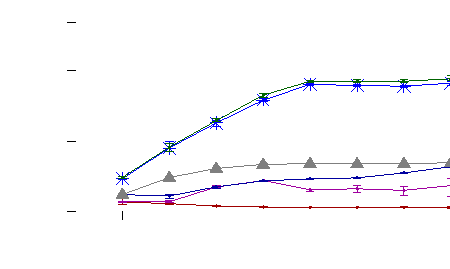
\includegraphics{new-malloc-test-1K-lutestring-aggregated}}%
    \gplfronttext
  \end{picture}%
\endgroup

\caption{A comparison of SuperMalloc, DLmalloc, Hoard,
  JEmalloc, and TBBmalloc running malloc-test
  on a 4-core (1 socket + hyperthreading) 3.4GHz i7-4770 (Haswell-DT)
  The lines are the average of 8 trials, and the error bars
  show the fastest and slow trial.}
\label{fig:datahtm}
\vspace*{-3ex}
\end{figure}

We originally designed the SuperMalloc for machines with HTM hardware.
We wanted to make it highly likely that the transactions would commit.
How well does the code run using pthread mutexes?  It turns out that
Glibc pthread mutexes are using hardware transactional memory on our
machine.  The performance with pthread mutexes is slightly slower than
running transactional memory, but the slowdown may not be significant.
We tried running the code using pthread mutexes on a Sandy Bridge
machine which does not have HTM\@.  \figref{datalock} shows the
results. This machine has 32 hardware threads, and so SuperMalloc
saturates the hardware at about 16 producer threads.  It turns out
that the same decisions that make HTM run fast also make lock-based
code run fast.

\begin{figure}
% GNUPLOT: LaTeX picture with Postscript
\begingroup
  \fontfamily{ptm}%
  \selectfont
  \makeatletter
  \providecommand\color[2][]{%
    \GenericError{(gnuplot) \space\space\space\@spaces}{%
      Package color not loaded in conjunction with
      terminal option `colourtext'%
    }{See the gnuplot documentation for explanation.%
    }{Either use 'blacktext' in gnuplot or load the package
      color.sty in LaTeX.}%
    \renewcommand\color[2][]{}%
  }%
  \providecommand\includegraphics[2][]{%
    \GenericError{(gnuplot) \space\space\space\@spaces}{%
      Package graphicx or graphics not loaded%
    }{See the gnuplot documentation for explanation.%
    }{The gnuplot epslatex terminal needs graphicx.sty or graphics.sty.}%
    \renewcommand\includegraphics[2][]{}%
  }%
  \providecommand\rotatebox[2]{#2}%
  \@ifundefined{ifGPcolor}{%
    \newif\ifGPcolor
    \GPcolortrue
  }{}%
  \@ifundefined{ifGPblacktext}{%
    \newif\ifGPblacktext
    \GPblacktextfalse
  }{}%
  % define a \g@addto@macro without @ in the name:
  \let\gplgaddtomacro\g@addto@macro
  % define empty templates for all commands taking text:
  \gdef\gplbacktext{}%
  \gdef\gplfronttext{}%
  \makeatother
  \ifGPblacktext
    % no textcolor at all
    \def\colorrgb#1{}%
    \def\colorgray#1{}%
  \else
    % gray or color?
    \ifGPcolor
      \def\colorrgb#1{\color[rgb]{#1}}%
      \def\colorgray#1{\color[gray]{#1}}%
      \expandafter\def\csname LTw\endcsname{\color{white}}%
      \expandafter\def\csname LTb\endcsname{\color{black}}%
      \expandafter\def\csname LTa\endcsname{\color{black}}%
      \expandafter\def\csname LT0\endcsname{\color[rgb]{1,0,0}}%
      \expandafter\def\csname LT1\endcsname{\color[rgb]{0,1,0}}%
      \expandafter\def\csname LT2\endcsname{\color[rgb]{0,0,1}}%
      \expandafter\def\csname LT3\endcsname{\color[rgb]{1,0,1}}%
      \expandafter\def\csname LT4\endcsname{\color[rgb]{0,1,1}}%
      \expandafter\def\csname LT5\endcsname{\color[rgb]{1,1,0}}%
      \expandafter\def\csname LT6\endcsname{\color[rgb]{0,0,0}}%
      \expandafter\def\csname LT7\endcsname{\color[rgb]{1,0.3,0}}%
      \expandafter\def\csname LT8\endcsname{\color[rgb]{0.5,0.5,0.5}}%
    \else
      % gray
      \def\colorrgb#1{\color{black}}%
      \def\colorgray#1{\color[gray]{#1}}%
      \expandafter\def\csname LTw\endcsname{\color{white}}%
      \expandafter\def\csname LTb\endcsname{\color{black}}%
      \expandafter\def\csname LTa\endcsname{\color{black}}%
      \expandafter\def\csname LT0\endcsname{\color{black}}%
      \expandafter\def\csname LT1\endcsname{\color{black}}%
      \expandafter\def\csname LT2\endcsname{\color{black}}%
      \expandafter\def\csname LT3\endcsname{\color{black}}%
      \expandafter\def\csname LT4\endcsname{\color{black}}%
      \expandafter\def\csname LT5\endcsname{\color{black}}%
      \expandafter\def\csname LT6\endcsname{\color{black}}%
      \expandafter\def\csname LT7\endcsname{\color{black}}%
      \expandafter\def\csname LT8\endcsname{\color{black}}%
    \fi
  \fi
  \setlength{\unitlength}{0.0500bp}%
  \begin{picture}(5760.00,3240.00)%
    \gplgaddtomacro\gplbacktext{%
      \csname LTb\endcsname%
      \put(640,558){\makebox(0,0)[r]{\strut{}\footnotesize 0}}%
      \csname LTb\endcsname%
      \put(640,1482){\makebox(0,0)[r]{\strut{}\footnotesize$50$M}}%
      \csname LTb\endcsname%
      \put(640,2407){\makebox(0,0)[r]{\strut{}\footnotesize$100$M}}%
      \csname LTb\endcsname%
      \put(640,2998){\makebox(0,0)[r]{\strut{}\footnotesize $132$M}}%
      \csname LTb\endcsname%
      \put(969,298){\makebox(0,0){\strut{} 1}}%
      \csname LTb\endcsname%
      \put(2036,298){\makebox(0,0){\strut{} 8}}%
      \csname LTb\endcsname%
      \put(3257,298){\makebox(0,0){\strut{} 16}}%
      \csname LTb\endcsname%
      \put(4477,298){\makebox(0,0){\strut{} 24}}%
      \csname LTb\endcsname%
      \put(5698,298){\makebox(0,0){\strut{} 32}}%
      \csname LTb\endcsname%
      \put(37,1796){\rotatebox{-270}{\makebox(0,0){\small \texttt{malloc()}'s per second}}}%
      \csname LTb\endcsname%
      \put(3287,19){\makebox(0,0){\small Producer threads}}%
      \put(3287,2942){\makebox(0,0){\strut{}}}%
      \csname LTb\endcsname%
      \put(3287,2941){\makebox(0,0){\strut{}}}%
      \colorrgb{0.00,0.39,0.00}%
      \put(3104,2776){\makebox(0,0)[r]{\strut{}\footnotesize SuperMalloc}}%
      \colorrgb{0.63,0.00,0.00}%
      \put(3562,669){\makebox(0,0)[r]{\strut{}\footnotesize DLmalloc}}%
      \colorrgb{0.63,0.00,0.63}%
      \put(5698,1575){\makebox(0,0)[r]{\strut{}\footnotesize Hoard}}%
      \colorrgb{0.00,0.00,0.63}%
      \put(3867,1575){\makebox(0,0){\strut{}\footnotesize JEmalloc}}%
      \colorrgb{0.00,0.63,0.63}%
      \put(3104,1390){\makebox(0,0)[r]{\strut{}\footnotesize TBBmalloc}}%
    }%
    \gplgaddtomacro\gplfronttext{%
    }%
    \gplbacktext
    \put(0,0){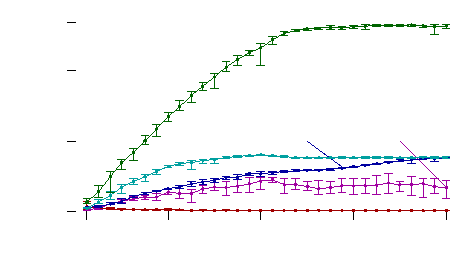
\includegraphics{new-malloc-test-1K-tempo-aggregated}}%
    \gplfronttext
  \end{picture}%
\endgroup

\caption{A comparison of SuperMalloc, DLmalloc \cite{Lea96}, Hoard
  \cite{BergerMcBl00}, and JEmalloc~\cite{Evans06} running malloc-test
  on a 16-core (2 sockets + hyperthreading) 2.4GHz E5-2665 (Sandy
  Bridge).  The lines are the average of 8 trials, and the error bars
  show the fastest and slow trial.}
\label{fig:datalock}
\vspace*{-3ex}
\end{figure}

We ran our experiments compiled with gcc 4.8.3 running on Linux 3.15.7
with glibc 2.18 on Fedora~20.  We compared SuperMalloc to Hoard 3.10,
jemalloc 3.6.0, and tbb43\_20140724.

\figref{variance} explores the variance of the allocators we measured
on the same experiment as for \figref{datahtm}.  We use the difference
between the slowest run and the fastest run as a measure of the
variance.  Not only are the newer allocators faster than DLmalloc, but
their variance is less.  In fact, the mean time to allocate for the
others is less than the variance of DLmalloc. For JEmalloc, TBBmalloc
and SuperMalloc, the worst-case time to allocate is less than the
variance of DLmalloc.  For all three of JEmalloc, TBBmalloc, and
SuperMalloc, the variance is similar, but since SuperMalloc runs about
three times faster, the relative variance is correspondingly three
times less.

\begin{figure}
\begin{center}
\begin{tabular}{l@{}rrrr}
            & Mean       & Fastest    & Slowest     & Diff       \\ \hline
DLmalloc    & \ns{340.8} & \ns{277.5} & \ns{428.8}  & \ns{151.4} \\
Hoard       & \ns{ 53.6} & \ns{ 41.8} & \ns{ 92.9}  & \ns{ 51.2} \\
JEmalloc    & \ns{ 31.1} & \ns{ 30.9} & \ns{ 31.5}  & \ns{  0.6} \\
TBBmalloc   & \ns{ 28.7} & \ns{ 28.4} & \ns{ 29.2}  & \ns{  0.8} \\
SuperMalloc & \ns{ 10.6} & \ns{ 10.4} & \ns{ 10.7}  & \ns{  0.4} \\
\end{tabular}
\end{center}
\caption{The speed of the each allocator, measured in time, for the
  8-thread case of \figref{datahtm}.  }
\label{fig:variance}
\end{figure}

The second important benchmark measured by \cite{Evans06} is Super
Smack.  Super Smack smacked us.  We were unable to get it to work.
We'll keep trying.

We tried running a few of the other benchmarks mentioned by
\cite{Evans06}.  Some of the benchmarks are difficult to reproduce,
and like Evans, we concluded that many of these benchmarks are not
very informative.  Here we discuss the ghostscript benchmark, as an example.

{\paragraph{gs:}} The gs benchmark was fairly easy to replicate, at
least in spirit.  There is a long history of running Ghostscript:
\cite{DetlefsDoZo94} ran it on an unspecified 126 page manual.
\cite{Evans06} ran it on an unspecified file named ``ps3.ps''.  So we
ran an unspecified file\footnote{If you really want to know, we used
  the 3251-page, 16,819,944-byte \cite{Intel13}.}  and ran it through
Ghostscript~9.14 as
\begin{minted}{sh}
$ gs -dBATCH -dNODISPLAY foo.pdf
\end{minted}
on a 4-core i7-4770 and saw the performance and maximum resident
memory (RSS) shown in \figref{gs}.  GS apparently allocates large
objects and runs its own allocator internally, mostly measuring the
behavior of large-object allocation.  The difference between DLmalloc
and TBBmalloc is small, less than one standard deviation.  SuperMalloc
is slightly slower, and the difference appears to be just larger than
the measurement error.  JEmalloc and TBBmalloc are significantly
slower; it is surprising that memory allocation can have such a large
performance impact, given that Ghostscript manages its own memory.
SuperMalloc is, by a small margin the most wasteful of space.
Interestingly, JEmalloc and Hoard, which are the slowest, also exhibit
the smallest memory footprint.

\begin{figure}
\begin{center}
\begin{tabular}{lrr}
            & Time$\pm\sigma$           & Max RSS \\              % user+system time                        maxrss
DLmalloc    & \unit{195.3\pm1.0}\second & \unit{150}\mebi\byte \\ % 195.27,194.66,194.13,197.30,194.35,194.90,196.30,195.24  153868 143516 146580 147180 151660 149424 143468 145276
Hoard       & \unit{212.9\pm0.6}\second & \unit{135}\mebi\byte \\ % 213.57,212.46,212.40,213.05,213.01,213.48,213.57,211.85  136396 138524 138524 138524 138524 138516 138524 138524
JEmalloc    & \unit{207.9\pm0.8}\second & \unit{129}\mebi\byte \\ % 207.86,206.86,206.69,207.66,209.11,208.26,207.93,208.57  129636 131996 132012 129656 129636 129660 131992 129660
TBBmalloc   & \unit{194.5\pm1.2}\second & \unit{158}\mebi\byte \\ % 194.53,197.07,193.58,193.43,194.07,194.72,193.15,195.18  156788 156788 159528 159520 161472 159532 161472 159528
SuperMalloc & \unit{197.3\pm1.4}\second & \unit{161}\mebi\byte \\ % 196.94,196.08,198.74,197.35,199.71,197.72,197.18,194.96  158128 164872 156340 158732 155588 166316 162832 155064

% elapsed Numbers from the big .ps
%DLmalloc 1:40.71
% eNumbers from the big .ps
%DLmalloc    & \unit{106.7\pm1.0}\second & \unit{283}\mebi\byte \\
%Hoard       & \unit{113.5\pm1.3}\second & \unit{289}\mebi\byte \\ %                   215.22                138520
%JEmalloc    & \unit{108.0\pm0.8}\second & \unit{291}\mebi\byte \\
%TBBmalloc   & \unit{105.9\pm0.4}\second & \unit{339}\mebi\byte \\ % time: 106.3 105.78 105.37 106.03  space: 347,336, 347,328, 347380, 347332,  mean=105.87 stddev=
%SuperMalloc & \unit{108.4\pm0.6}\second & \unit{346}\mebi\byte \\
\end{tabular}
\end{center}
\caption{The run time and maximum resident memory of running
  Ghostscript on \cite{Intel13}.  The run time is the average over
  eight runs with the standard deviation shown as a $\pm$.  The maximum
  resident memory is the maximum over the four runs.}
\label{fig:gs}
\end{figure}


{\paragraph{Larson:}} We ran the Larson benchmark \cite{LarsonKr98},
which is included in the Hoard distribution.  The Larson benchmark
simulates a server in which each thread allocates objects, keeps some
of them, eventually freeing them,, and passes some objects to other
threads where they will be freed.  We ran
\begin{minted}{sh}
./larson 10 7 500 1000 10000 1 8
\end{minted}
on a 4-core i7-4770 and saw the performance shown in \figref{larson}.
Instead of reporting throughput (which is operations per second), we
report time per operation, so that we can more easily compare averages
and standard deviations.  We also report standard deviation of the
time to call \code{malloc()}, and observe that the standard deviation
is much larger than the mean.  This means there are some very slow
allocations (the slowest allocations we measured took
\unit{81}\milli\second, and it wasn't clear that any of the allocators
has any particular advantage on this metric).  We were motivated by
the desire to reduce the slowest allocations, but it looks like we'll
have to embark on a study of much longer-running jobs to determine
whether we've made progress.  SuperMalloc was fastest by a small
margin.  This margin is much less than a standard deviation, but it
appears to be repeatable.

\begin{figure}
\begin{center}
\begin{tabular}{lrrr}
             & Mean Time/op            & $\sigma$              & Max RSS \\
DLmalloc     & \unit{1.72}\micro\second& \unit{50}\micro\second& \unit{6.6}\mebi\byte \\
Hoard        & \unit{1.57}\micro\second& \unit{38}\micro\second& \unit{7.0}\mebi\byte \\
JEmalloc     & \unit{1.47}\micro\second& \unit{40}\micro\second& \unit{8.7}\mebi\byte \\
TBBmalloc    & \unit{1.52}\micro\second& \unit{42}\micro\second& \unit{9.9}\mebi\byte \\
SuperMalloc  & \unit{1.42}\micro\second& \unit{39}\micro\second& \unit{7.3}\mebi\byte \\
\end{tabular}
\end{center}
\caption{The performance of the Larson benchmark.  The time per
  operation is the mean over four runs, with the standard deviation.
  The maximum resident memory is shown.  The malloc standard deviation
  is the variation among calls to \texttt{malloc()}.}
\label{fig:larson}
\end{figure}


{\paragraph{Footprint:}} The \defn{memory footprint} of an
application, the amount of physical memory that the application
consumes while running, can also vary by more than an order of
magnitude --- even a factor of two can be too much on something like a
database server where memory is used as a cache for disk, and an
increased footprint results in either a reduced effective cache size
or excessive I/O's due to paging.  We developed a benchmark based on
the idea of \cite{Vyukov08}, which operates by Thread~0 allocating
data and giving it to Thread~1 which frees the data.  Thread~1 then
allocates data and gives it to Thread~2, which frees the data.
Thread~2 then allocates and gives to Thread~3.  We configured the
vyukov benchmark to allocate 50,000 random objects per thread, each
object chosen to be a random size less than \unit{4}\kibi\byte, and
$200$ threads.  The application thus never asked for more than
\unit{100}\mebi\byte{} at a time.  The results are shown in
\figref{vyukov}.  Interestingly, DLmalloc and TBBmalloc both blew up
memory substantially, TBBmalloc nearly crashing our benchmark machine
in the process.  DLmalloc used \unit{2.3}\gibi\byte{} of RSS, and
TBBmalloc used \unit{4.1}\gibi\byte.  Also interesting is that
JEmalloc used a great deal of system time, apparently aggressively
calling \code{madvise()} to uncommit memory.

\begin{figure}
\begin{center}
\begin{tabular}{lrrrr}
           & User                & System              &  Elapsed             & MaxRSS \\
DLmalloc   & \unit{15.5}\second &  \unit{5.8}\second &  \unit{26.5}\second & \unit{2375}\mebi\byte \\
Hoard      & \unit{14.7}\second &  \unit{0.3}\second &  \unit{20.1}\second &  \unit{284}\mebi\byte \\
JEmalloc   & \unit{16.2}\second & \unit{10.3}\second &  \unit{30.6}\second &  \unit{228}\mebi\byte \\
TBBmalloc  & \unit{17.3}\second &  \unit{5.3}\second & \unit{111.3}\second & \unit{4214}\mebi\byte \\
SuperMalloc& \unit{16.0}\second &  \unit{0.2}\second &  \unit{21.3}\second &  \unit{219}\mebi\byte \\
\end{tabular}
\end{center}
\caption{The performance of the vyukov benchmark.  We measured the user time, system time, elapsed time, and max RSS.}
\label{fig:vyukov}
\end{figure}


{\paragraph{Complexity:}} A simple memory allocator can operate using
only a few hundred lines of code \cite{KernighanRi88}.  Since
allocator performance is so important, however, most allocators have
been tuned to run faster at the cost of increased complexity.  The
code sizes of \figref{codesize} show that SuperMalloc is smaller, but
where does the code complexity come from in these allocators?

\figref{supermodules} shows the largest modules in SuperMalloc.  The
biggest module is for managing the cache.  The interface to make the
standard POSIX calls is second biggest (including functions such as
reallocation, and testing).  The code for actually performing
allocation in the three size classes (small objects, medium/large objects, and huge objects)
together is just a little larger than the cache management code.  The
code for invoking locks or hardware transactional memory, and the
metaprogram that computes the bin sizes and sets up all the constants
are each also about 350 lines of code.  The code for interfacing to
mmap to get chunk-aligned memory is 123 lines.

\begin{figure}
\begin{center}
\begin{tabular}{lrr}
Module & Characters & LoC \\ \hline
mmap-interface         &   5,066 &  123 \\        
huge objects           &   7,312 &  189 \\
medium \& large objects&  10,203 &  302 \\
metaprogram            &  14,791 &  332 \\
atomicity and locks    &   9,296 &  357 \\
small objects          &  17,096 &  461 \\
Front end (API)        &  17,256 &  536 \\
Cache management       &  25,340 &  841 \\
\end{tabular}
\end{center}
\caption{The sizes of the significant modules of SuperMalloc, sorted by size.}
\label{fig:supermodules}
\end{figure}

For JEmalloc, the biggest module manages their ``arenas'' at 2,577
LoC, which implements the meat of their code, basically implementing
the functionality of our objects modules and the cache management
(which for us adds up to 1,793 LoC).  One significant module in
JEmalloc, in terms of lines of code, manages the tuning parameters
(giving the user control, for example, of the number of arenas and
providing access to various counters).  Although that code has many
lines of code, it is not complex.  It's just long because there are
many tuning parameters.  We do not want tuning parameters in
SuperMalloc, preferring instead that the code work well in all cases.
It may turn out that our determination to avoid tuning parameters will
fade away when faced with the demands of production --- we should
chalk up this part of JEmalloc's complexity to the fact that it's
production-quality code.

Hoard contains a huge number of modules, each of which is only a few
hundred lines of code, which can be used to build good special-purpose
and general-purpose allocators \cite{AlexandrescuBe05}.  SuperMalloc
isn't trying to enable to construction of special-purpose allocators,
so our code is smaller.

\secput{wishlist}{An Operating-System Wish List}

There are two features that Linux does not provide which are provided
by some other operating systems: a cheaper way to uncommit memory, and
a hook to reduce the odds that a thread is preempted while holding a
lock.  A third desirable feature, \defn{subscribable mutexes} does not
appear in any operating system, as far as we know.

{\paragraph{Cheap uncommit:}} The first problem is to uncommit memory
cheaply.  Linux provides a function
\begin{center}
\code{madvise(ptr, len, MADV_DONTNEED)}
\end{center}
which informs the operating system that the \code{len} bytes of memory
starting at address \code{ptr} are no longer needed.  For anonymously
mapped memory (the kind that \code{malloc()} uses), this removes the
page from the page table, freeing the physical page.  The next time
the process touches the page it will cause another page fault, at
which point the operating system will allocate and zero-fill a
physical page.  That is a fairly expensive operation --- it takes
\ns{1800} to call \code{madvise(MADV_DONTNEED)} to uncommit a page,
whereas if the page is already uncommited it costs only \ns{240} to
make the same system call.

One potential alternative is to use
\begin{center}
\code{madvise(ptr, len, MADV_FREE)},
\end{center}
which is provided by FreeBSD and Solaris.  The semantics of this call
is to give the kernel freedom to uncommit the page the way
\code{MADV_DONTNEED} does at any time until the process touches the
page again.  The kernel also has the freedom not to touch the page, so
that the data could still be the same data.  Since the kernel is in a
position to understand memory pressure as well as the overall system
load, it can decide when and whether to spend the CPU cycles to
reclaim memory.

Evans complains that ``\code{MADV_FREE} is \textit{way} nicer than
\code{MADV_DONTNEED} in the context of malloc.  JEmalloc has a really
discouraging amount of complexity that is directly a result of working
around the performance overhead of \code{MADV_DONTNEED}''
\cite{Evans12}.  We agree with Evans' sentiments, although the
SuperMalloc caches reduce the impact of the \code{madvise()} calls.
Although SuperMalloc would not get much simpler with \code{MADV_FREE},
it would speed up and exhibit less performance variance.

An alternative approach would be for the kernel to deliver an event to
a process indicating that it should use less memory.  The allocator
generally has a big list of empty pages lying around that it could
quickly return to the kernel.

{\paragraph{Lock-aware scheduling:}} The second problem shows up when
we are running in locking mode (that is, without transactional
memory).  Sometimes while a lock is held by a thread, the kernel
preempts the thread and schedules something else.  Since the thread
holds a lock, any other threads that try to acquire that lock suspend
too, which can lead to lock convoying and other performance problems.

Solaris provides one way to fix this using the \code{schedctl()}
system call, which tells the kernel not to, if possible, preempt a
thread for a little while\cite{Dice11}.  The mechanism includes two
steps: (1) the thread says it is about to enter a critical section,
and (2) the thread indicates that it has left the critical section.
Step (1) is accomplished by setting a bit in a thread-specific
structure.  Meanwhile the kernel, if it wanted to preempt the thread,
sets a bit in the structure.  Step (2) is accomplished by checking to
see if the ``wanted-to-preempt'' bit is set, and if so, politely
yielding.  The kernel must take some care to downgrade threads that
abuse the mechanism.

The Linux maintainers seem skeptical of this feature.  For example,
see \cite{Aziz14}, which proposed the patch and claimed that it
improves TPC-C performance by 3\%--5\%, but the kernel maintainers
dismissed it as ``a feature for a real-time kernel'' and suggested a
voluntary preemption model instead, and that they were ``skeptical
about the whole idea''.  One proposed \cite{Oboguev14a, Oboguev14b}
that a user-space mechanism to set the priority of a thread would solve
the problem.  As implementers of \code{malloc()}, we do not see how it
would --- \code{malloc()} is in a library, and we do not know what, if
any, thread priority schemes the application may be using.

We would like to see a hook in Linux to avoid preempting threads that
are briefly holding a lock.

{\paragraph{Subscribable mutexes:}} When running with HTM, we wait
until the lock used for the fallback path is not held, then we
subscribe to the lock.  It is not difficult to subscribe to the
pthread mutex lock in Linux, if you are willing to violate the POSIX
abstraction.  There is a single field in the mutex object that
indicates whether the lock is held.  It would better if the mutex
provided a way to subscribe to the lock abstractly.

A more difficult problem is what we should do when we are waiting for
a mutex to become free.  We do not want to spin indefinitely, but
there is no way to wait ask the operating system to wake us up when
the mutex becomes unlocked, except to lock the mutex.  What we need is
a way to wait for the mutex to become free without locking the mutex. 


%* Tradeoff: Code size and complexity, speed, footprint, variability.  Supermalloc appears to disprove this tradeoff.
%* Allocators use trees, buddy systems: supermalloc doesn't.
%* Work for HTM and locks.


\punt{
Notes: 
\begin{itemize}
%\item \cite{ReinefeldDoSc13} shows the importance of malloc.
% \item \cite{Dementiev09} shows an anecdote about the importance of caching even fairly large objects (200KiB).  He claims that the lazy-commit strategy was causing nonscalability.  I did an experiment, and it looks like his analysis is wrong (possibly superseded by newer kernels?)
%\item \cite{DetlefsDoZo94} Benchmarks include gs running on a 126-page manual.
%\item \cite{Michael04} shows a lock-free mallocator based on Hoard, with some interesting benchmarks: Linux-scalability, threadtest, larson and a producer-consumer test.
%\item \cite{FengBe05}
%\item \cite{SchneiderAnNi06}: streamflow (worries about cache behavior by using segregated heaps).  Synchronization-free operations for local alloc/free, and non-blocking synch for remote deallocations.  [In contrast, SuperMalloc doesn't care as much about trying to get cache behavior to be local.  Perhaps wrongly so.  Supermalloc does worry about false sharing  ].  Does poorly on memory footprint on the Larson benchmark, but they didn't isolate the issue, since they ran Larson for a fixed time instad of a fixed amount of work.
%\item \cite{LarsonKr98} LKmalloc hashes the threadid (so it doesn't need so many arenas, but it still needs a lock.)  They say for servers the requirements are to be fast, high-memory utilization, size indenpendent, locality, scalable, thread independence, predictable speed, stability).  LKmalloc is similar DLmalloc in that it uses bins of free blocks, approx best fit, and immediate coaslescing.  LKmalloc improves on DLmalloc by providing a lock per free list, multiple subheaps (to reduce cache sloshing (a value migrating around), select subheap by hasing, and striping (4MB pieces allocated to a heap)
%\item \cite{Gloger12} presents measurements of several allocators, with an emphasis on ptmalloc.
%\item \cite{Gloger06} is the web page for ptmalloc, an allocator based on dlmalloc \cite{Lea96}.
\item knary a benchmark we should use (since I helped write
  it...).  Knary was used in \cite{SchneiderAnNi06}, but was
  attributed to Hood when in fact it's due to \cite{BlumofeJoKu96}.
\end{itemize}
}



%SuperMalloc uses simple data structures to try to maximize the odds that hardware transactions succeed. For example, the SuperMalloc uses a priority heap to allocate objects out of the fullest page. The heap takes advantage of the fact that for each class, there are only a relatively small number of possible page-fullness values. For example, for 8-byte objects, there are only 512 objects in a page, and so instead of using a general heap, SuperMalloc uses an array of 513 lists, the $i$th list containing a list of pages with $i$ free slots.



%SuperMalloc uses a per-CPU cache and a per-thread cache. A per-thread cache of objects reduces the overhead of allocating and freeing objects because some objects do not need to perform any mutual exclusion. It turns out that most of the cost of updating a global data structure is due to cache misses, not the locking itself, however. On Haswell, an unlocked update to an uncontended cache line costs 3--5ns, whereas acquiring a lock and modifying uncontended variable costs 80ns. Acquiring an uncontended lock and updating an uncontended page costs only about 18ns. (On a multisocket Sandy Bridge processor, the difference is even more striking: 3ns uncontended unlocked, 26ns uncontended locked, and 460ns contended locked.) Accordingly, SuperMalloc uses a relatively small per-thread cache (containing only a few objects of each size), and uses a per-CPU cache (a cache per hardware thread). The per-CPU cache contains only one L3-cache worth of objects for each size class, since we assume that the application will actually store data into allocated objects. If the objects in the per-CPU cache don't fit in the L3 cache, then filling the objects will cause cache misses anyway, so it does not matter whether allocating the objects causes a few cache misses.

% To further improve the odds of transactions committing, SuperMalloc tries to prefetch into cache all the data of the transaction. Prefetching data appears to improve performance by about 5%.

%SuperMalloc appears to enjoy a substantially smaller footprint than the other allocators for two reasons. (1) SuperMalloc adopts Hoard's allocate-in-fullest-page heuristic rather than JEmalloc's approach of allocating the object with the lowest address. (2) SuperMalloc's caches are smaller than Hoard's or JEmallocs, mostly because the per-thread cache is extremely small, and in many applications there are far more threads than there are CPU's.

% SuperMalloc is currently implemented, and we are assembling and running the allocation benchmarks mentioned in other allocation papers. We plan to release the software under the Apache 2.0 license, and the assembled benchmarks under an appropriate mix of licenses.

\punt{
SuperMalloc, like Hoard, allocates objects out of the fullest possible page in order to reduce memory footprint.

madv\_dontneed (and other wishlists from the talk)

}

\secput{concl}{Conclusion}

SuperMalloc appears to be faster and more scalable than the other
scalable allocators.  Hoard and JEmalloc do pretty well under all
loads, whether you measure time, variance, or maximum RSS.
SuperMalloc starts faster and scales further, and uses less code.

We will soon release SuperMalloc under an open-source license.

{\raggedright
\bibliographystyle{abbrvnat}
\bibliography{allpapers}
}

%% \begin{figure*}
%% \begin{tabular}{cc}
%% % GNUPLOT: LaTeX picture with Postscript
\begingroup
  \fontfamily{ptm}%
  \selectfont
  \makeatletter
  \providecommand\color[2][]{%
    \GenericError{(gnuplot) \space\space\space\@spaces}{%
      Package color not loaded in conjunction with
      terminal option `colourtext'%
    }{See the gnuplot documentation for explanation.%
    }{Either use 'blacktext' in gnuplot or load the package
      color.sty in LaTeX.}%
    \renewcommand\color[2][]{}%
  }%
  \providecommand\includegraphics[2][]{%
    \GenericError{(gnuplot) \space\space\space\@spaces}{%
      Package graphicx or graphics not loaded%
    }{See the gnuplot documentation for explanation.%
    }{The gnuplot epslatex terminal needs graphicx.sty or graphics.sty.}%
    \renewcommand\includegraphics[2][]{}%
  }%
  \providecommand\rotatebox[2]{#2}%
  \@ifundefined{ifGPcolor}{%
    \newif\ifGPcolor
    \GPcolortrue
  }{}%
  \@ifundefined{ifGPblacktext}{%
    \newif\ifGPblacktext
    \GPblacktextfalse
  }{}%
  % define a \g@addto@macro without @ in the name:
  \let\gplgaddtomacro\g@addto@macro
  % define empty templates for all commands taking text:
  \gdef\gplbacktext{}%
  \gdef\gplfronttext{}%
  \makeatother
  \ifGPblacktext
    % no textcolor at all
    \def\colorrgb#1{}%
    \def\colorgray#1{}%
  \else
    % gray or color?
    \ifGPcolor
      \def\colorrgb#1{\color[rgb]{#1}}%
      \def\colorgray#1{\color[gray]{#1}}%
      \expandafter\def\csname LTw\endcsname{\color{white}}%
      \expandafter\def\csname LTb\endcsname{\color{black}}%
      \expandafter\def\csname LTa\endcsname{\color{black}}%
      \expandafter\def\csname LT0\endcsname{\color[rgb]{1,0,0}}%
      \expandafter\def\csname LT1\endcsname{\color[rgb]{0,1,0}}%
      \expandafter\def\csname LT2\endcsname{\color[rgb]{0,0,1}}%
      \expandafter\def\csname LT3\endcsname{\color[rgb]{1,0,1}}%
      \expandafter\def\csname LT4\endcsname{\color[rgb]{0,1,1}}%
      \expandafter\def\csname LT5\endcsname{\color[rgb]{1,1,0}}%
      \expandafter\def\csname LT6\endcsname{\color[rgb]{0,0,0}}%
      \expandafter\def\csname LT7\endcsname{\color[rgb]{1,0.3,0}}%
      \expandafter\def\csname LT8\endcsname{\color[rgb]{0.5,0.5,0.5}}%
    \else
      % gray
      \def\colorrgb#1{\color{black}}%
      \def\colorgray#1{\color[gray]{#1}}%
      \expandafter\def\csname LTw\endcsname{\color{white}}%
      \expandafter\def\csname LTb\endcsname{\color{black}}%
      \expandafter\def\csname LTa\endcsname{\color{black}}%
      \expandafter\def\csname LT0\endcsname{\color{black}}%
      \expandafter\def\csname LT1\endcsname{\color{black}}%
      \expandafter\def\csname LT2\endcsname{\color{black}}%
      \expandafter\def\csname LT3\endcsname{\color{black}}%
      \expandafter\def\csname LT4\endcsname{\color{black}}%
      \expandafter\def\csname LT5\endcsname{\color{black}}%
      \expandafter\def\csname LT6\endcsname{\color{black}}%
      \expandafter\def\csname LT7\endcsname{\color{black}}%
      \expandafter\def\csname LT8\endcsname{\color{black}}%
    \fi
  \fi
  \setlength{\unitlength}{0.0500bp}%
  \begin{picture}(5760.00,3240.00)%
    \gplgaddtomacro\gplbacktext{%
      \csname LTb\endcsname%
      \put(640,558){\makebox(0,0)[r]{\strut{}\footnotesize 0}}%
      \csname LTb\endcsname%
      \put(640,1482){\makebox(0,0)[r]{\strut{}\footnotesize$50$M}}%
      \csname LTb\endcsname%
      \put(640,2407){\makebox(0,0)[r]{\strut{}\footnotesize$100$M}}%
      \csname LTb\endcsname%
      \put(640,2998){\makebox(0,0)[r]{\strut{}\footnotesize $132$M}}%
      \csname LTb\endcsname%
      \put(969,298){\makebox(0,0){\strut{} 1}}%
      \csname LTb\endcsname%
      \put(2036,298){\makebox(0,0){\strut{} 8}}%
      \csname LTb\endcsname%
      \put(3257,298){\makebox(0,0){\strut{} 16}}%
      \csname LTb\endcsname%
      \put(4477,298){\makebox(0,0){\strut{} 24}}%
      \csname LTb\endcsname%
      \put(5698,298){\makebox(0,0){\strut{} 32}}%
      \csname LTb\endcsname%
      \put(37,1796){\rotatebox{-270}{\makebox(0,0){\small \texttt{malloc()}'s per second}}}%
      \csname LTb\endcsname%
      \put(3287,19){\makebox(0,0){\small Producer threads}}%
      \put(3287,2942){\makebox(0,0){\strut{}}}%
      \csname LTb\endcsname%
      \put(3287,2941){\makebox(0,0){\strut{}}}%
      \colorrgb{0.00,0.39,0.00}%
      \put(3104,2776){\makebox(0,0)[r]{\strut{}\footnotesize SuperMalloc}}%
      \colorrgb{0.63,0.00,0.00}%
      \put(3562,669){\makebox(0,0)[r]{\strut{}\footnotesize DLmalloc}}%
      \colorrgb{0.63,0.00,0.63}%
      \put(5698,1575){\makebox(0,0)[r]{\strut{}\footnotesize Hoard}}%
      \colorrgb{0.00,0.00,0.63}%
      \put(3867,1575){\makebox(0,0){\strut{}\footnotesize JEmalloc}}%
      \colorrgb{0.00,0.63,0.63}%
      \put(3104,1390){\makebox(0,0)[r]{\strut{}\footnotesize TBBmalloc}}%
    }%
    \gplgaddtomacro\gplfronttext{%
    }%
    \gplbacktext
    \put(0,0){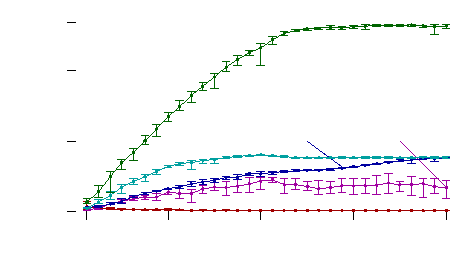
\includegraphics{new-malloc-test-1K-tempo-aggregated}}%
    \gplfronttext
  \end{picture}%
\endgroup

%% &
%% % GNUPLOT: LaTeX picture with Postscript
\begingroup
  \fontfamily{ptm}%
  \selectfont
  \makeatletter
  \providecommand\color[2][]{%
    \GenericError{(gnuplot) \space\space\space\@spaces}{%
      Package color not loaded in conjunction with
      terminal option `colourtext'%
    }{See the gnuplot documentation for explanation.%
    }{Either use 'blacktext' in gnuplot or load the package
      color.sty in LaTeX.}%
    \renewcommand\color[2][]{}%
  }%
  \providecommand\includegraphics[2][]{%
    \GenericError{(gnuplot) \space\space\space\@spaces}{%
      Package graphicx or graphics not loaded%
    }{See the gnuplot documentation for explanation.%
    }{The gnuplot epslatex terminal needs graphicx.sty or graphics.sty.}%
    \renewcommand\includegraphics[2][]{}%
  }%
  \providecommand\rotatebox[2]{#2}%
  \@ifundefined{ifGPcolor}{%
    \newif\ifGPcolor
    \GPcolortrue
  }{}%
  \@ifundefined{ifGPblacktext}{%
    \newif\ifGPblacktext
    \GPblacktextfalse
  }{}%
  % define a \g@addto@macro without @ in the name:
  \let\gplgaddtomacro\g@addto@macro
  % define empty templates for all commands taking text:
  \gdef\gplbacktext{}%
  \gdef\gplfronttext{}%
  \makeatother
  \ifGPblacktext
    % no textcolor at all
    \def\colorrgb#1{}%
    \def\colorgray#1{}%
  \else
    % gray or color?
    \ifGPcolor
      \def\colorrgb#1{\color[rgb]{#1}}%
      \def\colorgray#1{\color[gray]{#1}}%
      \expandafter\def\csname LTw\endcsname{\color{white}}%
      \expandafter\def\csname LTb\endcsname{\color{black}}%
      \expandafter\def\csname LTa\endcsname{\color{black}}%
      \expandafter\def\csname LT0\endcsname{\color[rgb]{1,0,0}}%
      \expandafter\def\csname LT1\endcsname{\color[rgb]{0,1,0}}%
      \expandafter\def\csname LT2\endcsname{\color[rgb]{0,0,1}}%
      \expandafter\def\csname LT3\endcsname{\color[rgb]{1,0,1}}%
      \expandafter\def\csname LT4\endcsname{\color[rgb]{0,1,1}}%
      \expandafter\def\csname LT5\endcsname{\color[rgb]{1,1,0}}%
      \expandafter\def\csname LT6\endcsname{\color[rgb]{0,0,0}}%
      \expandafter\def\csname LT7\endcsname{\color[rgb]{1,0.3,0}}%
      \expandafter\def\csname LT8\endcsname{\color[rgb]{0.5,0.5,0.5}}%
    \else
      % gray
      \def\colorrgb#1{\color{black}}%
      \def\colorgray#1{\color[gray]{#1}}%
      \expandafter\def\csname LTw\endcsname{\color{white}}%
      \expandafter\def\csname LTb\endcsname{\color{black}}%
      \expandafter\def\csname LTa\endcsname{\color{black}}%
      \expandafter\def\csname LT0\endcsname{\color{black}}%
      \expandafter\def\csname LT1\endcsname{\color{black}}%
      \expandafter\def\csname LT2\endcsname{\color{black}}%
      \expandafter\def\csname LT3\endcsname{\color{black}}%
      \expandafter\def\csname LT4\endcsname{\color{black}}%
      \expandafter\def\csname LT5\endcsname{\color{black}}%
      \expandafter\def\csname LT6\endcsname{\color{black}}%
      \expandafter\def\csname LT7\endcsname{\color{black}}%
      \expandafter\def\csname LT8\endcsname{\color{black}}%
    \fi
  \fi
  \setlength{\unitlength}{0.0500bp}%
  \begin{picture}(4320.00,2720.00)%
    \gplgaddtomacro\gplbacktext{%
      \csname LTb\endcsname%
      \put(538,558){\makebox(0,0)[r]{\strut{}\footnotesize 0}}%
      \csname LTb\endcsname%
      \put(538,1156){\makebox(0,0)[r]{\strut{}\footnotesize $50$M}}%
      \csname LTb\endcsname%
      \put(538,1694){\makebox(0,0)[r]{\strut{}\footnotesize $95$M}}%
      \csname LTb\endcsname%
      \put(809,298){\makebox(0,0){\strut{} 1}}%
      \csname LTb\endcsname%
      \put(1283,298){\makebox(0,0){\strut{} 2}}%
      \csname LTb\endcsname%
      \put(1758,298){\makebox(0,0){\strut{} 3}}%
      \csname LTb\endcsname%
      \put(2232,298){\makebox(0,0){\strut{} 4}}%
      \csname LTb\endcsname%
      \put(2706,298){\makebox(0,0){\strut{} 5}}%
      \csname LTb\endcsname%
      \put(3181,298){\makebox(0,0){\strut{} 6}}%
      \csname LTb\endcsname%
      \put(3655,298){\makebox(0,0){\strut{} 7}}%
      \csname LTb\endcsname%
      \put(4129,298){\makebox(0,0){\strut{} 8}}%
      \csname LTb\endcsname%
      \put(88,1359){\rotatebox{-270}{\makebox(0,0){\small \texttt{malloc()}'s per second}}}%
      \csname LTb\endcsname%
      \put(2516,19){\makebox(0,0){\small Producer threads}}%
      \put(2516,2440){\makebox(0,0){\strut{}\small 4-Core (8 hardware threads) 3.4GHz Haswell}}%
      \csname LTb\endcsname%
      \put(2516,2067){\makebox(0,0){\strut{}}}%
      \colorrgb{0.00,0.39,0.00}%
      \put(2090,1515){\makebox(0,0)[r]{\strut{}\footnotesize SuperMalloc}}%
      \colorrgb{0.63,0.00,0.00}%
      \put(2706,644){\makebox(0,0)[r]{\strut{}\footnotesize dlmalloc}}%
      \colorrgb{0.00,0.00,0.63}%
      \put(4082,678){\makebox(0,0)[r]{\strut{}\footnotesize Hoard}}%
      \colorrgb{0.63,0.00,0.63}%
      \put(4129,989){\makebox(0,0)[r]{\strut{}\footnotesize jemalloc}}%
    }%
    \gplgaddtomacro\gplfronttext{%
    }%
    \gplbacktext
    \put(0,0){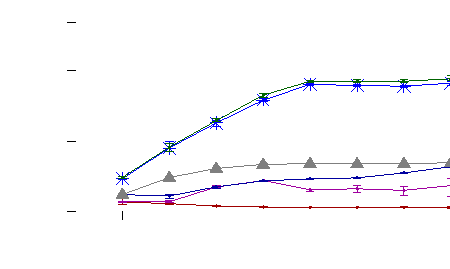
\includegraphics{new-malloc-test-1K-lutestring-aggregated}}%
    \gplfronttext
  \end{picture}%
\endgroup

%% \end{tabular}
%% \caption{A comparison of SuperMalloc, dlmalloc, Hoard, and jemalloc on the malloc-test benchmark.}
%% \label{fig:data}
%% \end{figure*}

\end{document}

%%  LocalWords:  SuperMalloc threadcount multithreaded implementers
%%  LocalWords:  allocator allocators JEmalloc HTM DLmalloc malloc ns
%%  LocalWords:  uncontended superblocks TBB TBBmalloc GPLv LKmalloc
%%  LocalWords:  superblock PTmalloc Cilk multithreading multicore
%%  LocalWords:  metadata unallocated uncommit madvise scalability
%%  LocalWords:  SuperMalloc's codesize mmap STL supermalloc Solaris
%%  LocalWords:  uncommited associativity rigamarole metaprogramming
%%  LocalWords:  incrementing prefetch deallocating prefetching Glibc
%%  LocalWords:  transactional atomicity uncommits dequeues pthread
%%  LocalWords:  mutexes Hyperthreading Ghostscript mutex POSIX
